%%%% Package Imports %%%%
\usepackage{algorithmicx}
\usepackage{amsmath, amsfonts, amscd, amssymb}
\usepackage{appendix}
\usepackage{array}
\usepackage{bigstrut}
\usepackage{blkarray}
\usepackage{color}
\usepackage{colortbl}
\usepackage{epsfig}
\usepackage{float}
\usepackage{framed}
\usepackage{gensymb}
\usepackage{graphicx}
\usepackage{hyperref}
\usepackage{import}
\usepackage{listings}
\usepackage{mathrsfs}
\usepackage{mathtools}
\usepackage{makeidx}
\usepackage{multicol}
\usepackage{multirow}
\usepackage{paralist}
\usepackage{relsize}
\usepackage{subcaption}
\usepackage{textcomp}
\usepackage{verbatim}
\usepackage{tikz}
\usepackage{xparse}
\usepackage{xcolor}
\usepackage{url}
\usepackage[plain]{algorithm}
\usepackage[noend]{algpseudocode}
\usepackage[customcolors]{hf-tikz}
\usepackage[framemethod=tikz]{mdframed}
 \usepackage{marginnote}
\usepackage{algorithm}%,algpseudocode}
\usepackage{mdframed}
\usepackage{longtable}
\usepackage{wasysym}
\usepackage[cc]{titlepic}
\usepackage{scalerel}

%%%% Color Definitions %%%%
\definecolor{red}{cmyk}{0, 1.00, 0.62,0}
\definecolor{blue}{cmyk}{1.00, .34, .0 .02 }    % blue
\definecolor{green}{cmyk}{0.7, 0, 1.0, 0.09 }   % greenish
\definecolor{yellow}{cmyk}{0, 0.16, 1.0, 0}     % yellow
\definecolor{gray}{cmyk}{0, 0, 0, 0.65}         % gray
\definecolor{purple}{cmyk}{.333, .867, 0, .059}
\colorlet{shadecolor}{blue!10}
\colorlet{warning}{red!20!}       %{RGB}{255, 188, 163}
\colorlet{warnline}{red}          %{RGB}{255, 15, 15}
\colorlet{information}{green!20}
\colorlet{infoline}{green}
\colorlet{codebase}{yellow!30!}
\colorlet{codekeyword}{blue}
\colorlet{codecomment}{green}
\colorlet{codestring}{red}
\colorlet{notgreen}{blue!50!yellow}

%%%% Length and Spacing %%%%
\setlength{\paperheight}{11in}
\setlength{\paperwidth}{8.5in}
\linespread{1.05}
\setlength{\parskip} {2pt plus1pt minus1pt}
 \setlength{\marg}{1.23in} %% Set the desired margin length here.

%%%% TikZ and Graphics %%%%
\usetikzlibrary{arrows, automata, backgrounds, calendar, chains, decorations,
\usetikzlibrary{circuits.ee.IEC}
\graphicspath{{figures/}{optimization/figures/figures-static/}}
\newcommand{\julia}{\raisebox{-.2\height}{
\includegraphics[scale = 0.07]{julia-logo}}  }
\newcommand{\jupyter}{\raisebox{-.2\height}{
\includegraphics[scale = 0.09]{jupyter-logo}}  }
\newcommand{\jump}{\raisebox{-.2\height}{
\includegraphics[scale = 0.08]{jump-logo}}  }
\newcommand{\gurobi}{\raisebox{-.2\height}{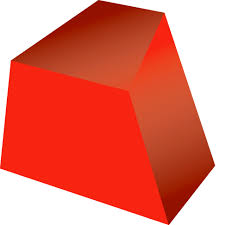
\includegraphics[scale = 0.06]{gurobi-logo}}Gurobi  }
\newcommand{\coin}{\raisebox{-.2\height}{
\includegraphics[scale = 0.2]{coin-or-logo}}  }

%%%% Math Commands %%%%
    \def\@pdfborder{0 0 1}
    \def\@pdfborderstyle{/S/U/W 1}
\renewcommand{\chaptername}{Lab}
\newcommand{\lab}[2]{\chapter[#2]{#1}}
\newcommand{\objective}[1]{{\bf Lab Objective: } \emph{#1} \bigskip}
\algnewcommand{\LineComment}[1]{\State \(\triangleright\) #1}
%\definecolor{shadecolor}{RGB}{186, 207, 188}
%\definecolor{information}{RGB}{235, 255, 223}
%\definecolor{infoline}{RGB}{69, 163, 11}
\mdfdefinestyle{problem}{backgroundcolor=shadecolor,
\lstdefinestyle{FromFile}{language=Python,
\lstdefinestyle{ShellOutput}{language=}
\lstdefinestyle{ShellInput}{language=}
\lstdefinestyle{pseudo}{basicstyle=\rmfamily,
\newcommand{\pseudoli}[1]{\lstinline[style=pseudo]!#1!}
\newcommand{\li}[1]{\lstinline[prebreak=]!#1!}
\newcommand{\lif}[1]{\lstinline[basicstyle=\footnotesize\ttfamily,language=Python,prebreak=]!#1!} % for inline code in footnotes.
\newcommand{\lsql}[1]{\lstinline[language=SQL,prebreak=,
\def\0{\mathbf{0}}
%\def\0{0}
\def\a{\mathbf{a}}
%\def\b{\mathbf{b}}
%\renewcommand{\b}{b}
%\def\b{b}
\def\c{\mathbf{c}}
\def\e{\mathbf{e}}
\def\f{\mathbf{f}}
\def\g{\mathbf{g}}
\def\p{\mathbf{p}}
\def\q{\mathbf{q}}
\def\u{\mathbf{u}}
\def\v{\mathbf{v}}
\def\w{\mathbf{w}}
\def\x{\mathbf{x}}
\def\y{\mathbf{y}}
\def\z{\mathbf{z}}
\def\subspace{\lhd}
\def\CalL{\mathcal{L}}
\def\CalO{\mathcal{O}}
\def\CalV{\mathcal{V}}
\def\CalU{\mathcal{U}}
\def\bU{{\bar{u}}}
\def\R{\Re e}
\def\I{\Im m}
\def\M{M_n}
\def\lvl#1{\multicolumn{1}{|c}{#1}} % Left  Vertical Line in array cell.
\def\rvl#1{\multicolumn{1}{c|}{#1}} % Right Vertical Line in array cell.
\renewcommand{\epsilon}{\varepsilon}                    % curly epsilon
\newcommand{\argmax}{\mbox{argmax}}
\newcommand{\indicator}{\boldsymbol{1}}
% \newcommand{\indicator}{\mathbbm{1}} % characteristic (indicator) function
\newcommand{\trp}{^{\mathsf T}}                         % matrix transpose
\newcommand{\hrm}{^{\mathsf H}}                         % hermitian conjugate
\newcommand{\ipt}[2]{\langle #1,#2 \rangle}
\newcommand{\ip}{\int_{-\infty}^{+\infty}}
\renewcommand{\ker}[1]{\mathcal{N}(#1)}
\newcommand{\ran}[1]{\mathcal{R}(#1)}
\newcommand\topstrut[1][0.8ex]{\setlength\bigstrutjot{#1}{\bigstrut[t]}}
\newcommand\botstrut[1][0.6ex]{\setlength\bigstrutjot{#1}{\bigstrut[b]}}
\newcommand{\Id}[1]{\mathrm{Id}(#1)}                    % Identity array
\newcommand{\makecopy}[1]{\mathrm{copy}(#1)}            % Copy an array
\newcommand{\shape}[1]{\mathrm{shape}(#1)}
\newcommand{\size}[1]{\mathrm{size}(#1)}
\DeclareMathOperator{\sign}{sign}
\DeclareMathOperator{\sech}{sech}
\DeclareMathOperator{\Out}{Out}                         % Used in PageRank lab
\DeclareMathOperator{\In}{In}                           % Used in PageRank lab
\DeclareMathOperator\erf{erf}
\newcommand{\contributor}[2]{\noindent\vtop{\hsize14pc#1\\\itshape#2}\par}
%\newcommand{\cr}[1]{\mathbf{#1}} % change to \mathbb
\newcommand{\rc}{\cellcolor{red}} % change cell color red in table
\newcommand{\hi}{\cellcolor{red}} % change cell color red in table
%\def\input@path{{/figures/}}
%\def\input@path{{/path/to/folder/}{/path/to/other/folder/}}
\renewcommand{\thealgsubstate}{\alph{algsubstate}}
   \renewcommand{\State}{%
\newcommand\hcancel[2][0.5pt]{%
\newcommand{\tblue}[1]{{\color{blue} #1}}
\newcommand{\tred}[1]{{\color{red} #1}}
\newcommand{\tgreen}[1]{{\color{notgreen} #1}}
\newcommand{\code}[1]{\texttt{ #1}}
\newcommand{\complexity}[1]{{\color{red} \textit{#1}}}
\newcommand{\nphard}{\complexity{NP-Hard}}
\newcommand{\npcomplete}{\complexity{NP-Complete}}
\newcommand{\polynomial}{{\color{ansi-green} \textit{Polynomial time (P)}}}
\newcommand{\true}{\tgreen{\texttt{ true }}}
\newcommand{\false}{\tred{\texttt{ false }}}
\newcommand{\ipopt}{\raisebox{-.2\height}{\texttt{Ipopt}}}
\def \PP{ {\mathcal{P}}}
\def \NN{ {\mathcal{N}}}
\def \II{ {\mathcal{I}}}
\def \ZZ{ {\mathcal{Z}}}
\def \SS{ {\mathcal{S}}}
\def \FF{ {\mathcal{F}}}
\def \CC{ {\mathcal{C}}}
\def \nn{ {\mathbb{N}}}
\def \R{ {\mathbb{R}}}
\def \Z{ {\mathbb{Z}}}
\def \Q{ {\mathbb{Q}}}
\def \cc{ {\mathbb{C}}}
\DeclareMathOperator{\dom}{dom}
\DeclareMathOperator{\cl}{cl}
\DeclareMathOperator{\intr}{intr}
\def \rank{\textup{rank}}
\def \size{\textup{size}}
%\def \dist{\textup{dist}}
\def \sign{\textup{sign}}
\def \deg{\textup{deg}}
\def \conv{\textup{conv}}
\def \cone{ {\textup{cone}}}
\def \supp{\textup{supp}}
\def \int{ {\textup{int}}}
\def \rc{\textup{rec.cone}}
\def \ri{\textup{rel.int}}
\def \rb{ {\textup{rel.bd}}}
\def \bd{ {\textup{bd}}}
\def \ls{\textup{lin.space}}
\def \tq{{\,:\,}}
\def \aff{{\textup{aff}}}
\def \one{\mathbb{1}}
\def \st{ \text{ s.t. }}
\def \BQP{\mathrm{BQP}}
\def \xLP{x^{\mathrm{LP}}}
\DeclareMathOperator    \argmin         {arg\,min}
%\DeclareMathOperator    \argmax         {arg\,max}
\protected@edef\@currentlabelname{Exercise \theexo: #1}% addition here
\protected@edef\@currentlabelname{Code}% addition here
  \protected@edef\@currentlabelname{#1}
  \protected@edef\@currentlabelname{Example \theexo}
  \protected@edef\@currentlabelname{Example \theexo}
  \protected@edef\@currentlabelname{Example \theexo}
  \protected@edef\@currentlabelname{Example \theexo}
\newcommand{\floor}[1]{\lfloor #1 \rfloor}
\newcommand{\ceil}[1]{\lceil #1 \rceil}
\newcommand{\mathup}[1]{#1}
\newcommand{\NP}{\text{NP}}
\newcommand{\coNP}{\text{coNP}}
\newcommand{\lift}{\mathrm{lift}}
\newcommand{\ub}{\mathrm{ubbest}}
\newcommand{\F}{{\mathcal F}}

%%%% Algorithm Environments %%%%
\restylefloat{algorithm}
     \Statex {\footnotesize\thealgsubstate:}\space}}

%%%% Custom Commands and Environments %%%%
%\newenvironment{problem}{\begin{mdframed}[style=problem]\begin{problemnum}}{\end{problemnum}\end{mdframed}}
%\newenvironment{problem*}{\begin{mdframed}[style=problem]\begin{problemnum*}}{\end{problemnum*}\end{mdframed}}
\newenvironment{contributors}{{List of Contributors}%
\newenvironment{algsubstates}
\newenvironment{exo}[1]%
\newenvironment{codeCell}%
\newenvironment{general}[2]
  \newenvironment{optexample}
   \newenvironment{examplewithcode}[2]
   \newenvironment{examplewithallcode}[4]
   \newenvironment{examplewithoutcode}[2]

%%%% General Settings %%%%
\g@addto@macro\@floatboxreset\centering
\Hy@AtBeginDocument{

%%%% Miscellaneous %%%%
    matrix, mindmap, patterns, petri, positioning, shadows, shapes.geometric,
    trees, shapes, decorations.pathreplacing}
\hfsetfillcolor{red!02}
\hfsetbordercolor{red}
\makeatletter
\@addtoreset{footnote}{chapter}
\makeatother
\floatstyle{ruled}
\makeatletter
}
\makeatother
 \newlength{\marg}
                        skipabove=10pt,
                        skipbelow=10pt
                        leftmargin=20pt,
                        rightmargin=20pt,
                        innertopmargin=10pt,
                        innerbottommargin=10pt,
                        innerleftmargin=10pt,
                        middlelinewidth=0pt,
                        everyline=true,
                        linecolor=blue,
                        linewidth=2pt}
\newmdenv[
  skipabove=10pt
  skipbelow=10pt
  leftmargin=20pt,
  rightmargin=20pt,
  backgroundcolor=warning,
  innertopmargin=10pt,
  innerbottommargin=10pt,
  innerleftmargin=10pt,
  middlelinewidth=0pt,
  everyline=true,
  linecolor=warnline,
  linewidth=2pt,
  font=\normalfont\normalsize,
  frametitlefont=\large\bfseries,
  frametitleaboveskip=1em,
  frametitlerule=true,
  frametitle={\sc Caution!}
]{warn}
\newmdenv[
  skipabove=10pt,
  skipbelow=10pt,
  leftmargin=20pt,
  rightmargin=20pt,
  backgroundcolor=information,
  outerlinewidth=0pt,
  outerlinecolor=infoline,
  innertopmargin=10pt,
  innerbottommargin=10pt,
  innerleftmargin=10pt,
  middlelinewidth=0pt,
  everyline=true,
  linecolor=infoline,
  linewidth=2pt,
  font=\normalfont\normalsize,
  frametitlefont=\large\bfseries,
  frametitleaboveskip=1em,
  frametitlerule=true,
  frametitle={\sc Note}
]{info}
\lstset{
  language=Python,
  backgroundcolor=\color{codebase},   %\color[RGB]{250, 245, 182},
  tabsize=4,
  basewidth=.5em,
  rulecolor=\color{yellow},           %\color{black},
  basicstyle=\normalsize\ttfamily,    % code text size
  upquote=true,
  columns=fixed,
  extendedchars=true,
  breaklines=true,
  prebreak = \raisebox{0ex}[0ex][0ex]{\ensuremath{\hookleftarrow}},
  frame=lrtb,
  xleftmargin=5pt,
  xrightmargin=5pt,
  framesep=4pt,
  framerule=2pt,
  showtabs=false,
  showspaces=false,
  showstringspaces=false,
  morestring=[s]{"""}{"""},
  morestring=[s]{'''}{'''},
  keywordstyle=\color{codekeyword},   %\color[RGB]{42, 161, 152},
  commentstyle=\color{codecomment},   %\color[RGB]{108, 153, 8},
  stringstyle=\color{codestring},     %\color[RGB]{189, 78, 98},
  title=\lstname,
  captionpos=b,
  abovecaptionskip=-5pt,
  belowcaptionskip=-5pt,
  moredelim=[is][\color{black}]{<<}{>>},
  moredelim=[is][\color{red}]{<r<}{>r>},
  moredelim=[is][\color{blue}]{<b<}{>b>},
  moredelim=[is][\color{green}]{<g<}{>g>},
  moredelim=[is][\color{purple}]{<p<}{>p>},
  morekeywords={assert, bytes, self, super, with, as, yield, True, False, None, NotImplemented, BaseException, Exception, AssertionError, AttributeError, ImportError, IndexError, KeyError, KeyboardInterrupt, MemoryError, NameError, NotImplementedError, OSError, OverflowError, RecursionError, RuntimeError, StopIteration, SyntaxError, IndentationError, TabError, StandardError, SystemError, SystemExit, TypeError, ValueError, ZeroDivisionError, IOError, Warning, RuntimeWarning, FileExistsError, FileNotFoundError,
    SELECT, FROM, AS, INNER, JOIN, LEFT, OUTER,
    CROSS, ON, WHERE, CASE, IF,
    MIN, MAX, SUM, AVG, COUNT,
    TEXT, REAL
  },
  deletekeywords={compile, format}
}
                          frame=single,
                          numbers=left,
                          numberstyle=\tiny,
                          stepnumber=2,
                          numbersep=7pt,
                          numberfirstline=true,
                          abovecaptionskip=2pt,
                          belowcaptionskip=2pt
                          }
                        upquote=true,
                        keywordstyle=\color{black}\bfseries,
                        commentstyle=\color[rgb]{0.133,0.545,0.133},
                        stringstyle=\color[rgb]{0.627,0.126,0.941},
                        }
                                morekeywords={TEXT, REAL, IF}]!#1!}
\providecommand{\abs}[1]{\left\lvert#1\right\rvert}
\providecommand{\norm}[1]{\left\lVert#1\right\rVert}
\providecommand{\set}[1]{\lbrace#1\rbrace}
\providecommand{\setconstruct}[2]{\lbrace#1:#2\rbrace}
\NewDocumentCommand\allocate{m+g}{                      % Empty array
  \IfNoValueTF{#2}
    {\mathrm{empty}(#1)}                                % 1 dimension
    {\mathrm{empty}(#1, #2)}                            % 2 dimensions
}
\NewDocumentCommand\zeros{m+g}{                         % Zero array
  \IfNoValueTF{#2}
    {\mathrm{zeros}(#1)}
    {\mathrm{zeros}(#1, #2)}%
}
             \thispagestyle{plain}\begin{multicols}{2}\parindent0pt%
\parskip6pt plus2pt minus1pt%
\widowpenalty10000\clubpenalty10000}
               {\end{multicols}   
               This project is funded in part by the National Science Foundation, grant no. TUES Phase II DUE-1323785.            
               \clearpage}
\cellcolor{red}
\newtheorem{ICE}{ICE}%[section]
\newcounter{algsubstate}
  {\setcounter{algsubstate}{0}%
     \stepcounter{algsubstate}%
  {}
\numberwithin{equation}{section}
\newsavebox\CBox
  \ifmmode\sbox\CBox{$#2$}\else\sbox\CBox{#2}\fi%
  \makebox[0pt][l]{\usebox\CBox}%  
  \rule[0.5\ht\CBox-#1/2]{\wd\CBox}{#1}}
\newcounter{general}
  \newcounter{exo}
{\refstepcounter{exo}%
\vspace{0.5cm}\noindent
{\large\bfseries{Exercise \theexo~: #1} \par}
{\par\vspace{0.5cm}}}
\newcounter{codeCell}
{\refstepcounter{codeCell}%
{}
{}}
  {\par\medskip
   \begin{framed}
   \begingroup\color{black}%
   \textbf{#1: }\ignorespaces
   \par #2
   \par}
 {\endgroup\end{framed}
  \medskip}
  {\par\medskip
  \refstepcounter{exo}%
   \begin{framed}
   \begingroup\color{blue}%
   \textbf{Example \theexo: }\ignorespaces}
 {\endgroup\end{framed}
  \medskip}
  {\par\medskip
   \refstepcounter{exo}%
  \begin{center}
 \rule{\textwidth}{0.4pt}\\
 \vspace{-0.2cm}
 \rule{\textwidth}{0.4pt}
 \end{center}
   \begingroup\color{black}%
   \textbf{Example: #1}
   \hfill \protect\href{#2}{Gurobipy}% code link somehow
    \ignorespaces
    \par}
 { \endgroup
   \begin{center}
 \rule{\textwidth}{1.8pt}
 \end{center}
  \medskip}
  {\par\medskip
   \refstepcounter{exo}%
   \begin{framed}
   \begingroup\color{black}%
   \textbf{Example: #1}
   \hfill \protect\href{#2}{ \ Excel \ }\protect\href{#3}{ \ PuLP \ }\protect\href{#4}{\ Gurobipy \ }% code link somehow
    \ignorespaces
    \par}
 { \endgroup
 \end{framed}
  \medskip}
  {\par\medskip
   \refstepcounter{exo}%
   \begin{framed}
   \begingroup\color{black}%
   \textbf{Example: #1}
    \ignorespaces
    \par}
 { \endgroup
 \end{framed}
  \medskip}
